\documentclass[10pt,twocolumn]{article}

% arXiv-ready, Overleaf-trivial: only standard packages, manual bibliography.
% Layout follows the conventions of Springer research articles (two columns, sans-serif
% numbered headings, "Fig. N" captions below figures, "Table N" captions above tables,
% booktabs rules, a full-width abstract). The text block is 7.0in wide, which is exactly
% the width the figures are authored at, so \includegraphics never rescales them.
\usepackage[a4paper,left=0.635in,right=0.635in,top=0.95in,bottom=1.0in,
            columnsep=0.28in]{geometry}
\usepackage[T1]{fontenc}
\usepackage[utf8]{inputenc}
\usepackage{mathptmx}          % Times body text + matching math
\usepackage[scaled=0.92]{helvet} % Helvetica for the sans-serif headings
\usepackage{courier}
\usepackage{amsmath,amssymb}
\usepackage{natbib}
\usepackage{graphicx}
\usepackage{booktabs}
% lightweight siunitx substitutes (avoids the texlive-science dependency)
\newcommand{\percent}{\%}
\newcommand{\num}[1]{#1}
\newcommand{\SI}[2]{#1\,#2}
\newcommand{\SIrange}[3]{#1--#2\,#3}
\usepackage{xcolor}
% Links are live but restrained: a dark navy that stays legible in greyscale print
% rather than the default saturated blue/green/red, which looks unfinished.
\definecolor{linknavy}{HTML}{1A4C7C}
\usepackage[colorlinks=true,linkcolor=linknavy,citecolor=linknavy,urlcolor=linknavy,
            breaklinks=true]{hyperref}
% Document properties: without these the PDF ships with blank Title/Author/Keywords, which
% is what indexers and reference managers read.
\hypersetup{
  pdftitle={How Much of DeFi Liquidity Is Higher-Order? Survivorship, LP Representation,
            and Structural Stability},
  pdfauthor={Adam Levine},
  pdfsubject={Higher-order network structure of Ethereum stablecoin liquidity: survivorship
              de-censoring, LP-token representation sensitivity, and structural stability
              across two stress events},
  pdfkeywords={decentralised finance; higher-order networks; persistent homology;
               survivorship bias; automated market makers; nerve complex; JEL: C81, D85,
               C65, E42, G14, G23},
  pdfcreator={pdfTeX}}
% Clickable external identifiers for the bibliography. The visible text stays the bare
% DOI / arXiv id, so the reference is still complete on paper.
\newcommand{\doi}[1]{\href{https://doi.org/#1}{doi:#1}}
\newcommand{\arxiv}[1]{\href{https://arxiv.org/abs/#1}{arXiv:#1}}
\usepackage[font=small,labelfont=bf,labelsep=space]{caption}
\usepackage{titlesec}
\usepackage{fancyhdr}
\usepackage{microtype}

\renewcommand{\figurename}{Fig.}

% Narrow (3.35in) columns plus unbreakable \texttt{} endpoint names and URLs otherwise
% leave a handful of very loose lines. Let TeX break inside typewriter text and spend a
% little emergency stretch rather than gapping the interword spaces.
\tolerance=1200
\setlength{\emergencystretch}{2.2em}
\renewcommand{\UrlBreaks}{\do\/\do\.\do\-\do\_\do\a\do\c\do\e\do\g\do\i\do\m\do\o\do\p\do\t}

% Five full-width floats in a six-page two-column paper: with LaTeX's defaults they queue
% up and the last one lands on a float-only page at the end. Let a top float own most of
% the page and allow two per page, so each figure appears on or near the page that
% discusses it.
\renewcommand{\dbltopfraction}{0.92}
\renewcommand{\dblfloatpagefraction}{0.5}
\renewcommand{\topfraction}{0.9}
\renewcommand{\bottomfraction}{0.7}
\renewcommand{\textfraction}{0.07}
\renewcommand{\floatpagefraction}{0.7}
\setcounter{dbltopnumber}{3}
\setcounter{topnumber}{3}
\setcounter{totalnumber}{4}

% Springer-style headings: sans-serif bold, number then space, no trailing period.
\titleformat{\section}{\sffamily\bfseries\large}{\thesection}{0.7em}{}
\titleformat{\subsection}{\sffamily\bfseries\normalsize}{\thesubsection}{0.6em}{}
\titleformat{\paragraph}[runin]{\sffamily\bfseries}{}{0pt}{}
\titlespacing*{\section}{0pt}{1.6ex plus .3ex}{0.8ex}
\titlespacing*{\subsection}{0pt}{1.3ex plus .3ex}{0.5ex}
\titlespacing*{\paragraph}{0pt}{1.2ex plus .2ex}{0.5em}

\pagestyle{fancy}
\fancyhf{}
\fancyhead[L]{\footnotesize\itshape How much of DeFi liquidity is higher-order?}
\fancyhead[R]{\footnotesize\thepage}
\renewcommand{\headrulewidth}{0.4pt}
\renewcommand{\headrule}{\color{black!35}\hrule height 0.4pt}

\begin{document}

\twocolumn[
\begin{@twocolumnfalse}
\vspace*{-0.5cm}
{\raggedright
{\sffamily\bfseries\LARGE How Much of DeFi Liquidity Is Higher-Order?\\[3pt]
Survivorship, LP Representation, and Structural Stability\par}
\vspace{1.2em}
{\sffamily\large Adam Levine\par}
\vspace{0.45em}
{\small Department of Economics, Hofstra University\ \ \textperiodcentered\ \
\texttt{adalevine08@gmail.com}\par}
\vspace{0.35em}
{\footnotesize Preprint, \today\par}
}

\vspace{1.6em}
% NB: no \\[..] at brace level 0 in here -- the ] would close \twocolumn's optional arg.
{\noindent\sffamily\bfseries Abstract\par}
\vspace{0.35em}
\noindent{\small
How much of the loop structure of a DeFi liquidity network is genuinely higher-order, and
is that quantity stable? Curve's 3pool binds $\{$USDC,\,USDT,\,DAI$\}$ in a single
contract, a three-way relationship a pairwise graph discards and the \emph{nerve complex}
of pool co-membership keeps. Measured over Ethereum stablecoin
pools by persistent homology, the quantity is \textbf{representation-dependent}: the
higher-order fraction spans \num{0.31} to \num{0.93} across two defensible modeling
choices that are rarely reported as sensitivities. The larger driver is \textbf{LP-token
representation}. Resolving an LP token such as 3CRV into its base assets collapses
metapools toward a cone and roughly doubles the fraction; keeping 3CRV as its own vertex
does not. The second driver is \textbf{survivorship}, and it is fixable. Standard
registry-based reconstruction filters today's pool list backwards, silently conditioning
on survival, and recovers only $\sim$\SI{10}{\percent} of the loop structure. Internet
Archive snapshots of the registry endpoint recover the rest: we rebuild the full
historical universe over \num{36} snapshots (Oct 2022 to May 2025). De-censoring also
revives the LP-resolution comparison, untestable on survivors alone since those
metapools have all delisted. Once those two choices are separated, the structure itself is
\textbf{stable} under every remaining variation we test. Through both the March 2023 USDC
depeg and the July 2023 Curve/Vyper exploit an event window is indistinguishable from an
arbitrary window of equal length, under either representation and on either sample. We
bound that stability rather than assert it. Synthetic damage shows the measure tracks how
many pools die, not how much value: a shock had to eliminate about a fifth of the universe
to register, and the depeg delisted 15 pools holding \SI{0.8}{\percent} of TVL. An
apparent signal at the exploit traced to corrupted TVL in the one archive crawl captured
mid-event, and repairing it removes the signal. That is a second data-quality trap beside
survivorship, and registry-based work has to guard against it. We read the stability
economically: stablecoins are
common-numéraire substitutes, so their liquidity scaffold is shallow and does not re-wire
under price stress. The methodological lesson is to report
the higher-order content of a DeFi network as a sensitivity range over survivorship and
representation, never as a point estimate. Code and data are fully reproducible.
\par}

\vspace{0.9em}
\noindent{\small{\sffamily\bfseries Keywords}\ \ Decentralised finance \textperiodcentered\
Higher-order networks \textperiodcentered\ Persistent homology \textperiodcentered\
Survivorship bias \textperiodcentered\ Automated market makers\par}

\vspace{0.5em}
\noindent{\small{\sffamily\bfseries JEL classification}\ \ C81 \textperiodcentered\ D85
\textperiodcentered\ C65 \textperiodcentered\ E42 \textperiodcentered\ G14
\textperiodcentered\ G23\par}
\vspace{1.8em}
\end{@twocolumnfalse}
]

\section{Introduction}

Classical financial-contagion models are pairwise: institutions are nodes, bilateral
exposures are edges \citep{eisenberg2001}. A multi-asset AMM pool is not. Curve's 3pool
binds $\{$USDC, USDT, DAI$\}$ into one contract, and a graph records only the three
pairwise projections, discarding the joint membership. Higher-order network methods
(hypergraphs, simplicial complexes; \citealp{bick2023}) retain exactly that information,
and a nascent literature argues they matter for systemic risk \citep{forte2026}. The
decisive reason to test this in decentralised finance rather than traditional finance is
\textbf{observability}: pool compositions and reserves are public and machine-readable
on-chain, removing the confidentiality barrier that has always constrained structural
contagion research.

We make ``how much is higher-order?'' a measurement. For each snapshot we build the nerve
complex of pool co-membership and compute the \emph{skeleton-vs-nerve decomposition}: the
cycle rank of the 1-skeleton ($E-V+B_0$, the loops a graph sees) vs.\ the Betti-1 number
$B_1$ of the nerve (loops surviving once multi-asset pools fill their faces). Their
ratio is the fraction of loop structure that is genuinely higher-order.

The central finding is that this fraction is \textbf{a property of the representation as
much as of the network}. Two knobs that any such study must set, and that are rarely
reported as sensitivities, move it from a clear minority to an overwhelming majority:

\begin{enumerate}
\item \textbf{LP-token representation.} A Curve metapool reads nominally as
$\{X, \text{3CRV}\}$. Resolving 3CRV into its underlying $\{$USDC,\,USDT,\,DAI$\}$ makes
every such pool a simplex containing the 3pool triangle as a face, pushing the complex
toward a cone (contractible, higher-order by construction); keeping 3CRV as its own vertex
does not. This choice is the \emph{larger} driver.
\item \textbf{Survivorship.} The standard historical reconstruction filters
\emph{today's} registry back in time, so it silently conditions on pools that survived,
disproportionately the large multi-asset pools. This inflates the higher-order fraction
and, we show, is fixable.
\end{enumerate}

Our contributions:
\begin{itemize}
\item \textbf{A de-censoring method for DeFi registry survivorship} (\S\ref{sec:data}):
Internet-Archive snapshots of the registry recover the full historical universe,
delisted pools included. Survivor-only reconstruction captures $\sim$1/10 of the loops
(\S\ref{sec:cnt}); the method applies to any registry-based DeFi network study.
\item \textbf{A sensitivity decomposition of the higher-order fraction}
(\S\ref{sec:frac}): it spans \num{0.31}--\num{0.93} across representation $\times$
survivorship; we separate the two contributions and show even the \emph{sign of the
time-trend} is convention-dependent. De-censoring revives the otherwise-untestable
LP-resolution fork.
\item \textbf{Structural stability across two events} (\S\ref{sec:null}): the reconstructed
structure is stable through \emph{both} the USDC depeg and the Curve/Vyper exploit under
every choice we vary. It is the one representation- and sample-independent structural
statement the data supports. Establishing it required a second data-quality guard: an integrity scan
plus transient-dip repair that removes a spurious signal from the corrupted archive crawl
captured mid-exploit.
\end{itemize}

A rigorous negative on the dynamics, and a demonstration that the descriptive metric is an
artifact, together map where higher-order topology does and does not add value over
pairwise methods, which we did not know in advance.

\section{Related work}

\textbf{Higher-order finance} is early-stage. \citet{forte2026} give the first hypergraph
analysis of bank--firm credit networks (Central Bank of Argentina registry, adjusted
H-eigenvector centrality): TradFi credit and centrality, not persistent homology and not
DeFi. \textbf{Return-space TDA} is by contrast saturated: persistent homology of return
point clouds covers equities \citep{gidea2018}, FX, and crypto \citep{fx2025}; we keep this
lineage strictly separate, as our complex is built from \emph{structure} (co-membership),
not return correlation. \textbf{Graph analysis of DeFi} exists: \citet{uniswap2025} model
Uniswap as a token-node/pool-edge network, exactly the pairwise baseline our
decomposition sits atop; \citet{tradefidefi2025} survey the surrounding systemic-risk
literature. To our knowledge the persistent-homology / nerve treatment of DeFi liquidity
structure is previously unoccupied, and, more to the point, the survivorship and
representation sensitivities we quantify are not addressed in registry-based DeFi network
work, which typically reconstructs history from the current registry without either
control.

\section{Data: the registry, and de-censoring its survivorship}
\label{sec:data}

\begin{figure*}[t]
\centering
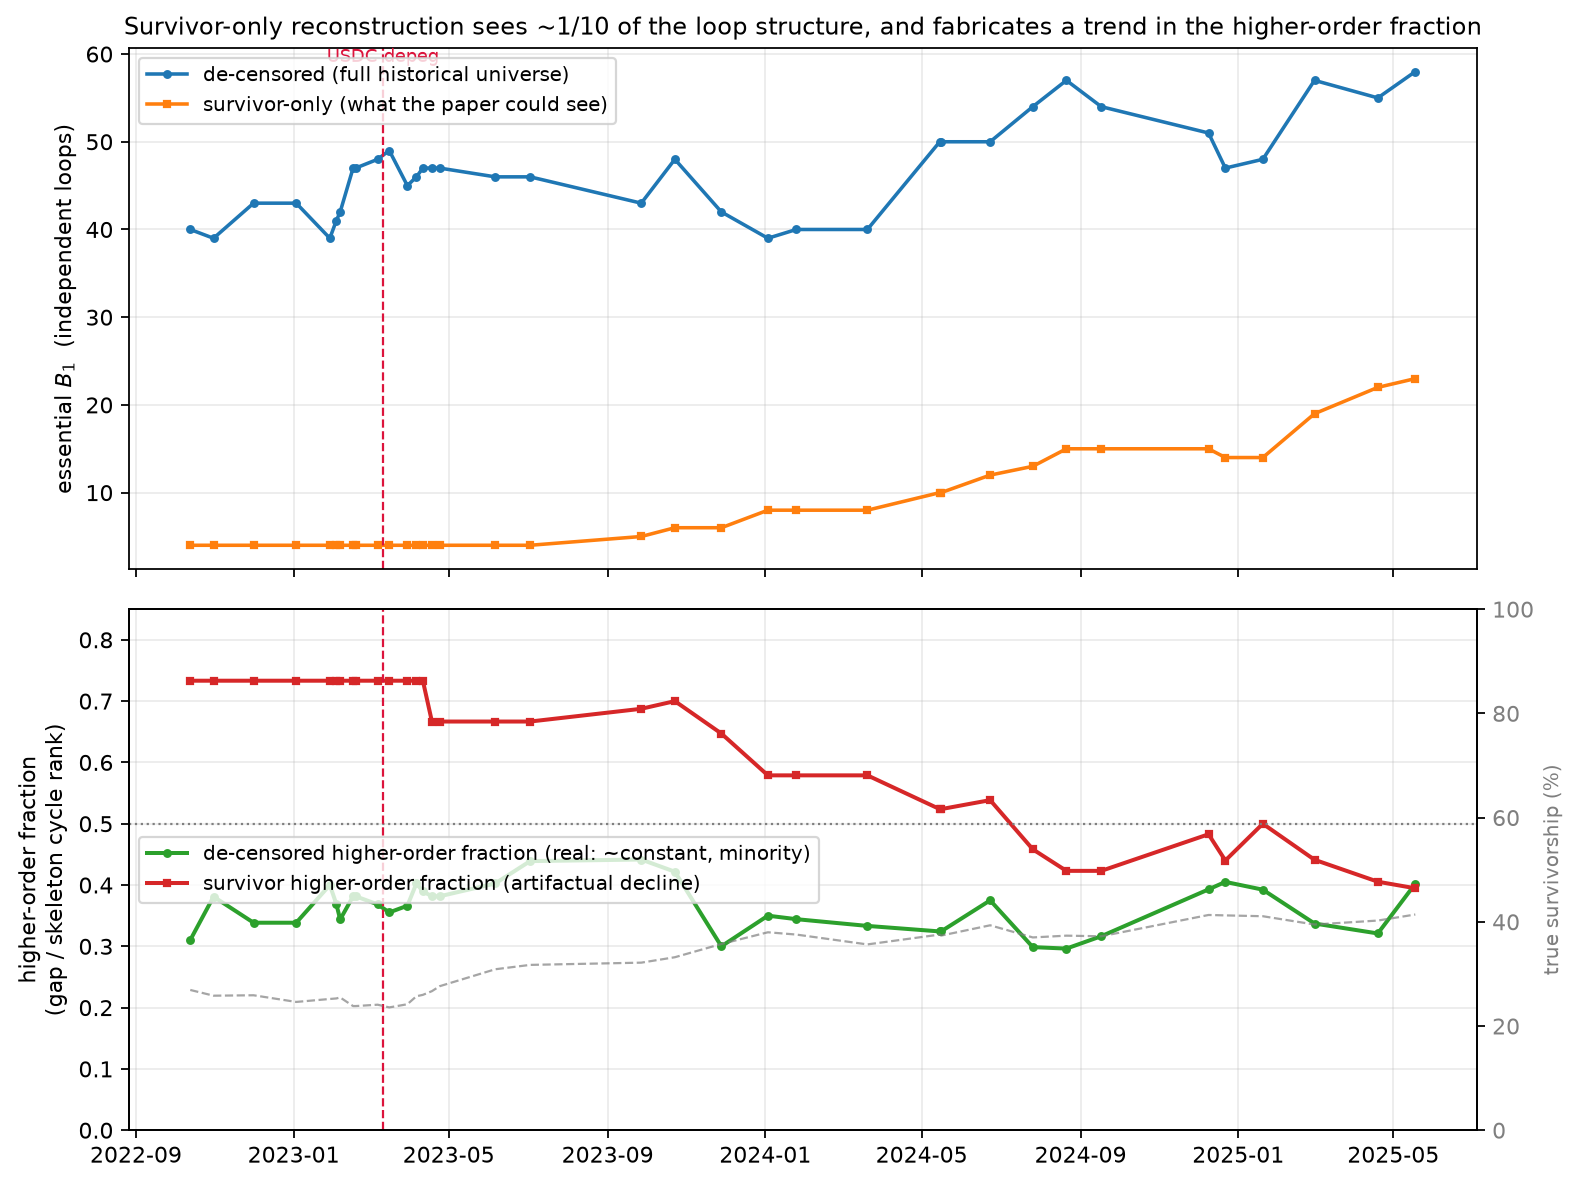
\includegraphics[width=\textwidth]{decensor.png}
\caption{Survivor-only reconstruction sees roughly one loop in ten, and manufactures a
trend that is not there. \textbf{a} Essential $B_1$ on the de-censored full historical
universe (blue) vs.\ on pools that survive to today (red); the shaded wedge is the loop
structure a survivor-only study cannot see. \textbf{b} The higher-order fraction is flat on
the full universe (green) but declines on survivors (red), and that decline tracks the
rising survivorship rate (grey, right axis): it is the survivor sample converging to
the truth, not the network changing. Vertical line: the USDC depeg (2023-03-11).}
\label{fig:decensor}
\end{figure*}

We use two free, unauthenticated DeFiLlama endpoints: the pool registry
(\texttt{yields.llama.fi/pools}: project, chain, symbol, \texttt{underlyingTokens},
current TVL, stablecoin flag) and per-pool daily TVL history
(\texttt{yields.llama.fi/chart/\{pool\}}). The universe is Ethereum, stablecoin-flagged
pools with $2$--$8$ underlying tokens.

\paragraph{The standard reconstruction, and its hidden conditioning.} Since a pool's
token set is fixed at deployment, the usual historical complex at date $t$ is today's
registry filtered to pools with TVL above threshold at $t$. This silently conditions on
survival: pools delisted before today are invisible. It has been treated (including in two
independent reviews of an earlier draft of this work) as an \emph{unrecoverable} ceiling.

\paragraph{De-censoring.} It is not unrecoverable. The Wayback Machine archived the
registry endpoint roughly weekly from October 2022; each snapshot is the \emph{full}
universe at that date, delisted pools included, with the identical schema. We fetch
\num{42} archived crawls (Oct 2022--May 2025, monthly, with tight clusters around the
USDC depeg and the July 2023 Curve/Vyper exploit); \num{36} of these form the primary
monthly series and the remaining six are the event clusters. We rebuild the complex on the full
historical universe, and, per snapshot, also restrict to pools surviving to today,
isolating the survivorship effect at fixed representation. True survivorship rises from
\SI{24}{\percent} to \SI{41}{\percent} over the period (mechanically: recent pools are
likelier to persist); at the depeg only 66 of 274 universe pools survive, and the 208
invisible pools were \SI{35}{\percent} of universe TVL (FRAX-3CRV \$474M,
MIM/OUSD/TUSD/LUSD-3CRV, \ldots). Terra (May 2022) predates the archive and is not
de-censorable; snapshots are weekly crawl dates, not daily. One caveat we make operational
below: a crawl captured during an acute event can carry corrupted TVL, so snapshots are run
through an integrity scan (\S\ref{sec:null}).

\section{Method}
\label{sec:method}

\paragraph{Complex and filtration.} Vertices are tokens (by contract address); a pool with
token set $\sigma$ contributes the filled simplex on $\sigma$ (downward closure). We
filter by each pool's \emph{share} of universe TVL at date $t$, entering strong pools first
at $f=-\log_{10}(\text{share})$, a level-invariant weighting, so a result cannot be the
mechanical TVL drawdown of a depeg in disguise. We track $B_0$, essential $B_1$, $B_2$
($\equiv 0$ throughout), the 1-skeleton cycle rank $E-V+B_0$, and the higher-order
fraction $\text{HO} = (E-V+B_0-B_1)/(E-V+B_0)$. Topology code is validated on
hand-checkable toy complexes (a hollow triangle has one loop, a filled one none, a
tetrahedron boundary has $B_2=1$).

\paragraph{Why essential $B_1$ and not persistence summaries.} The filtration above
supports the standard return-space TDA summaries (persistence landscapes, $L^p$ norms,
total persistence) and we do not use them, for a reason worth stating. On this object
almost every $H_1$ class is essential: across all \num{42} crawls under both
representations, \num{35} of \num{3430} $H_1$ classes have finite persistence
($1.0$\percent), never more than two on a single crawl against 40--58 essential ones; on
the daily survivor-only series the rate is exactly zero across 579 consecutive days. Under
the discard-infinite convention that \texttt{gudhi} and the return-space pipeline use by
default, the $H_1$ landscape is therefore identically zero or near enough. Capping infinite
bars instead makes the norms non-zero, but they then track the arbitrary cutoff rather than
the data, and event and placebo windows stay indistinguishable ($L^2$ 1.22 vs.\ 1.25).
$H_0$ is the control: it has genuine finite bars and the machinery works there. The reason
is structural, not numerical --- a loop here closes only if some pool contains all of its
tokens, which weaker pools entering later do not do --- so the vanishing is specific to $H_1$
on a co-membership complex. We read this as a transferable caution: the return-space TDA
toolkit does not carry to structural liquidity complexes, and Betti numbers are the
appropriate summary.

\paragraph{The two modeling axes.} We cross \textbf{sample} (survivor-only vs.\
de-censored/full) with \textbf{LP representation}: \emph{lp\_vertex} keeps LP tokens as
their own vertices (the archive's native form), \emph{resolved} replaces the 3CRV LP token
(identified as \texttt{0x6c3f\ldots e490}, present in $\sim$68 metapools per snapshot in
the archive) with $\{$DAI,\,USDC,\,USDT$\}$. Today's API base-resolves, so the survivor
reconstruction is implicitly the \emph{resolved} fork; the archive's native form makes
\emph{lp\_vertex}, and with it the comparison, available for the first time.

\paragraph{Event test and data-quality guard.} With snapshots at weekly cadence we test
each event non-parametrically: is the pre$\to$post change large relative to the
distribution of all consecutive-snapshot changes across the series? We run two events (the
USDC depeg, 2023-03-07 $\to$ 03-16; the Curve/Vyper exploit, 2023-07-30 $\to$ 08-02) under
both representations. Since a crawl captured mid-event can be corrupted, every snapshot
first passes an \emph{integrity scan} (flag if universe TVL is $<0.6\times$ the median of
its temporal neighbours); a flagged snapshot's \emph{transient dips} (pools materially
live on both neighbours but $<0.5\times$ the smaller on the flagged crawl) are repaired by
neighbour interpolation, the snapshot-level analogue of the daily gap-fill. (An earlier
daily survivor-only analysis using a placebo-window permutation test over 632 daily
complexes reaches the same result; we report the de-censored version as primary evidence.)

\section{Results}

\subsection{Survivor reconstruction sees $\sim$1/10 of the loop structure}
\label{sec:cnt}

At fixed representation (lp\_vertex), essential $B_1$ is \textbf{40--58 on the full
universe vs.\ 4--23 on survivors}, at every snapshot; the true universe is 3--4$\times$
the survivor universe (234--430 vs.\ 63--178 pools). The object a survivor-only study
analyses is a small, biased slice, and the bias is toward exactly the large multi-asset
pools that dominate the higher-order fraction.

\subsection{The higher-order fraction is a modeling artifact}
\label{sec:frac}

\begin{figure*}[t]
\centering
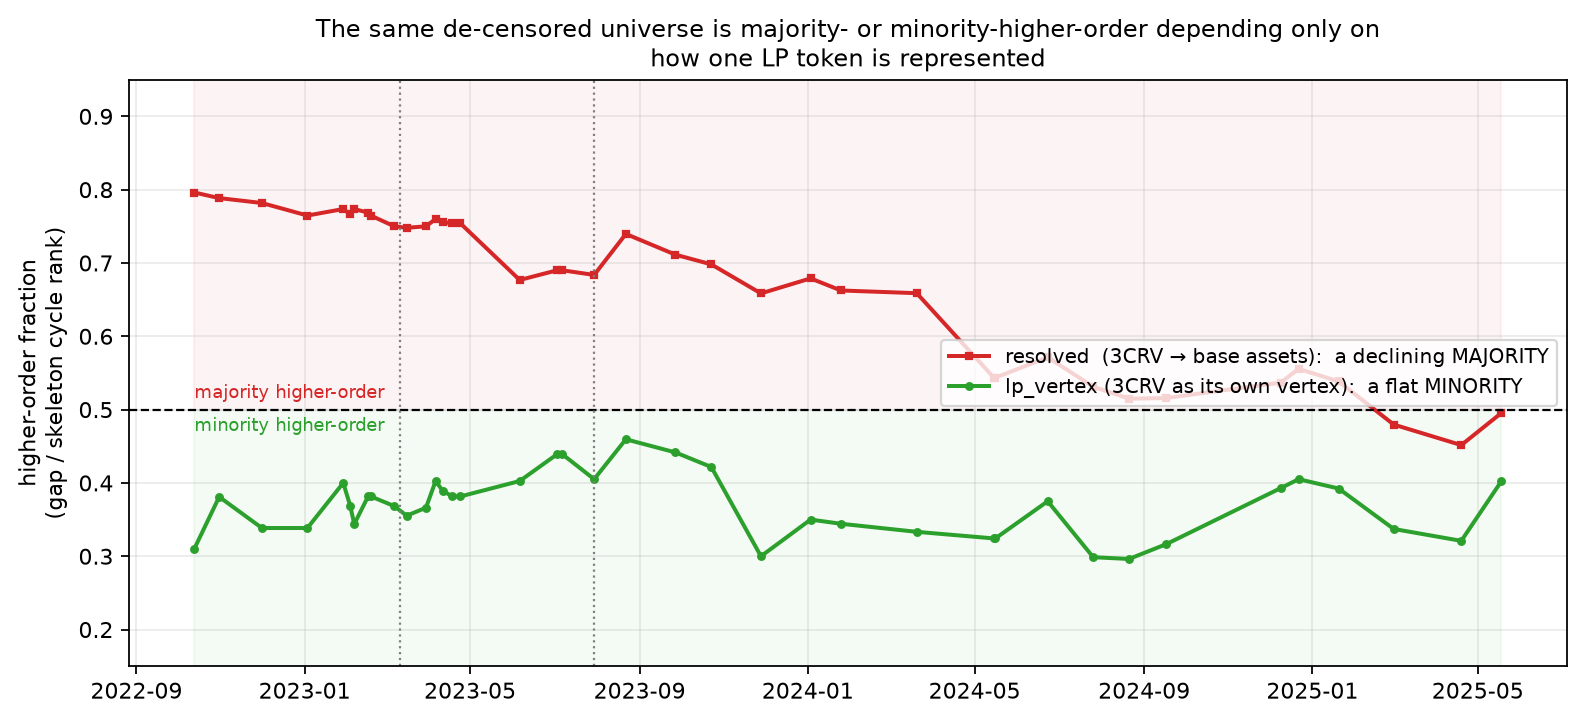
\includegraphics[width=\textwidth]{representation.png}
\caption{The \emph{same} de-censored universe reads as majority- or minority-higher-order
purely by LP-token representation. Resolving 3CRV to base assets (red squares) keeps the
fraction a declining majority ($>0.5$); keeping 3CRV as its own vertex (green circles)
keeps it a flat minority ($<0.5$). The shaded band between them is the span of one
modelling choice that is rarely reported; the two conventions sit on opposite sides of the
majority line for the entire period, converging only as the metapool structure dissolves.
The corrupted 2023-08-02 crawl (Sec.~\ref{sec:null}) is excluded.}
\label{fig:repr}
\end{figure*}

Table~\ref{tab:2x2} crosses the two axes. The higher-order fraction spans
\textbf{0.31--0.93}. Reading it two ways:

\begin{table*}[t]
\centering
\caption{Higher-order fraction by sample $\times$ LP representation. The paper-standard
corner (resolved, survivor) reads a declining majority; the de-censored,
composability-preserving corner (lp\_vertex, full) reads a flat minority. Same data.}
\label{tab:2x2}
\small
\begin{tabular}{lcccc}
\toprule
snapshot & lp\_vertex, full & lp\_vertex, survivor & resolved, full & resolved, survivor \\
\midrule
2022-10 & 0.31 & 0.73 & 0.80 & 0.93 \\
2023-03 & 0.37 & 0.73 & 0.75 & 0.93 \\
2023-06 & 0.40 & 0.67 & 0.68 & 0.92 \\
2023-11 & 0.30 & 0.65 & 0.66 & 0.87 \\
2024-05 & 0.32 & 0.52 & 0.54 & 0.77 \\
2024-12 & 0.39 & 0.48 & 0.54 & 0.68 \\
2025-05 & 0.40 & 0.39 & 0.50 & 0.60 \\
\bottomrule
\end{tabular}
\end{table*}

\begin{itemize}
\item \textbf{Representation is the larger driver.} Resolving 3CRV collapses $\sim$68
metapools onto a shared base triangle (a partial cone): across \num{36} snapshots it
removes $\sim$\SI{28}{\percent} of loops (essential $B_1$ $46.8\to33.8$) yet nearly
\emph{doubles} the higher-order fraction ($0.36\to0.67$). At the depeg, full-universe HO is
\num{0.37} (lp\_vertex) vs.\ \num{0.75} (resolved).
\item \textbf{Survivorship amplifies in the same direction.} Holding representation =
resolved (the paper-standard convention), full$\to$survivor pushes HO $0.75\to0.93$ at the
depeg, since survivors are the big multi-asset pools.
\item \textbf{Even the trend is convention-dependent} (Fig.~\ref{fig:decensor}). Under
resolved, the de-censored fraction genuinely \emph{declines} $0.80\to0.50$ as metapools
delist; under lp\_vertex it is \emph{flat} at $0.36\pm0.04$. The survivor fraction declines
under both, but that is the survivor sample converging to the full-universe value as
survivorship rises (corr(survivor HO, survivorship) $=-0.92$ for lp\_vertex), not a change
in the network.
\end{itemize}

So the paper-standard ``a majority of loops are higher-order, declining over 2022--23''
sits at the high-inflation corner; the de-censored, composability-preserving reading is a
flat minority (Fig.~\ref{fig:repr}). Both conventions are economically defensible
(resolving reflects exposure to base assets; lp\_vertex reflects composability structure),
but they are not symmetric in kind. Resolving carries a mechanical inflation that
lp\_vertex has no counterpart for: each metapool becomes a filled simplex sharing the 3pool
triangle, adding one vertex and three edges to a common base, so the skeleton cycle rank
rises by two while $B_1$ does not move. The gap widens by construction, $\sim$68 times
over. Under lp\_vertex the same pool is a single edge on a star centred at 3CRV and adds
nothing to either quantity. What lp\_vertex costs is interpretive rather than mechanical:
a holder of FRAX-3CRV is exposed to four assets and lp\_vertex records a two-asset
relationship. Only one of the two conventions manufactures the quantity being measured,
which is worth saying plainly even though it does not pick a winner.
\textbf{The appropriate estimand is therefore a sensitivity range over representation and
sample (Table~\ref{tab:2x2}), reported as such rather than collapsed to a point value.}

\subsection{Structural stability across stress events}
\label{sec:null}

With the representation and sample choices made explicit, the structure itself is stable,
and stays stable on a second event and after data-quality control. Table~\ref{tab:null} runs the de-censored event test on
both events. Two details of the test matter enough to state. First, crawl spacing is
irregular (1--83 days, median 26) while the event windows are 9 and 3 days, and drift grows
with the gap --- mean $|\Delta|$ in essential $B_1$ is 1.40 on intervals of $\le$14 days
against 2.44 across all intervals --- so judging an event against the full pair list would
bias the comparison toward finding no change. We therefore match on spacing. Second, the
observables are small integers, so $|\Delta|$ ties heavily and the percentile depends on
whether ties are counted below or at the event value; on the depeg that choice alone moves
essential $B_1$ from the 23rd to the 49th percentile. We use the mid-rank convention
throughout. Under both corrections the events land near the \emph{median} of comparable
routine intervals rather than in the lower tail: the sharper statement is that an event
window is indistinguishable from an arbitrary window of the same length, not that it is
unusually quiet.

\begin{table}[t]
\centering
\caption{De-censored event test, full universe, both events. $|\Delta|$ is the change
across the event window (depeg 2023-03-07 $\to$ 03-16, 9 days; exploit 2023-07-30 $\to$
08-02, 3 days, after transient-dip repair). Percentiles are mid-rank against
\emph{gap-matched} reference intervals ($\le$14 days, $n=15$), not all 41 consecutive
pairs, whose median spacing is 26 days and whose drift is correspondingly larger.
``Detect'' is the largest routine change observed across those 15 intervals, which is what
the 95th percentile resolves to at this $n$: the size of move the test can separate from
normal variation. Both events sit near the middle of
routine variation for comparable windows, and well under the threshold, under both
representations.}
\label{tab:null}
\small
\setlength{\tabcolsep}{4.5pt}
\begin{tabular}{llccc}
\toprule
observable & repr. & \multicolumn{1}{c}{$|\Delta|$} & pct. & detect \\
 & & \multicolumn{1}{c}{\scriptsize depeg / expl.} & & \\
\midrule
ess.\ $B_1$ & lp\_vertex & 1 / 1 & 53rd & 5 \\
gap         & lp\_vertex & 1 / 1 & 47th & 7 \\
ess.\ $B_1$ & resolved   & 0 / 0 & 27th & 4 \\
gap         & resolved   & 1 / 1 & 50th & 11 \\
\bottomrule
\end{tabular}
\end{table}

\paragraph{A second event, and a data-quality trap.} The Curve/Vyper exploit (2023-07-30)
at first appears to show a response: on the de-censored universe essential $B_1$ jumps
$47\to55$ (90th percentile) under lp\_vertex and $31\to37$ under resolved. But the integrity
scan flags the single 08-02 crawl as the \emph{only} anomaly in the series (universe TVL
halves, $\$3.04$B$\to\$1.73$B, then recovers), and 84\% of that drop is 10
transient-dipped registry rows (6 distinct pools; DeFiLlama re-lists the same Curve pool
under Convex), 8 of them FRAX (FRAX-USDC $\$435$M$\to\$73$M$\to\$451$M; FRAX-USDP
$\$112$M$\to\$3$M$\to\$129$M): corrupted readings during the exploit, not a real drawdown
(the exploit drained \$70M of \emph{ETH} pools, not stablecoins). Repairing the transient
dips removes the signal entirely: essential $B_1$ returns to 48, its pre-event value
(Fig.~\ref{fig:curve}), and the Curve window is stable. The result therefore holds on
\textbf{$N=2$} events, each confirmed only after snapshot data QC. The episode is itself a
result: \emph{archived registry snapshots crawled during acute events can manufacture
spurious topological signals. It is a second data-quality trap beside survivorship, and
one an unguarded pipeline would have reported as the sought-after ``topology detects the
exploit'' finding.}

\begin{figure*}[t]
\centering
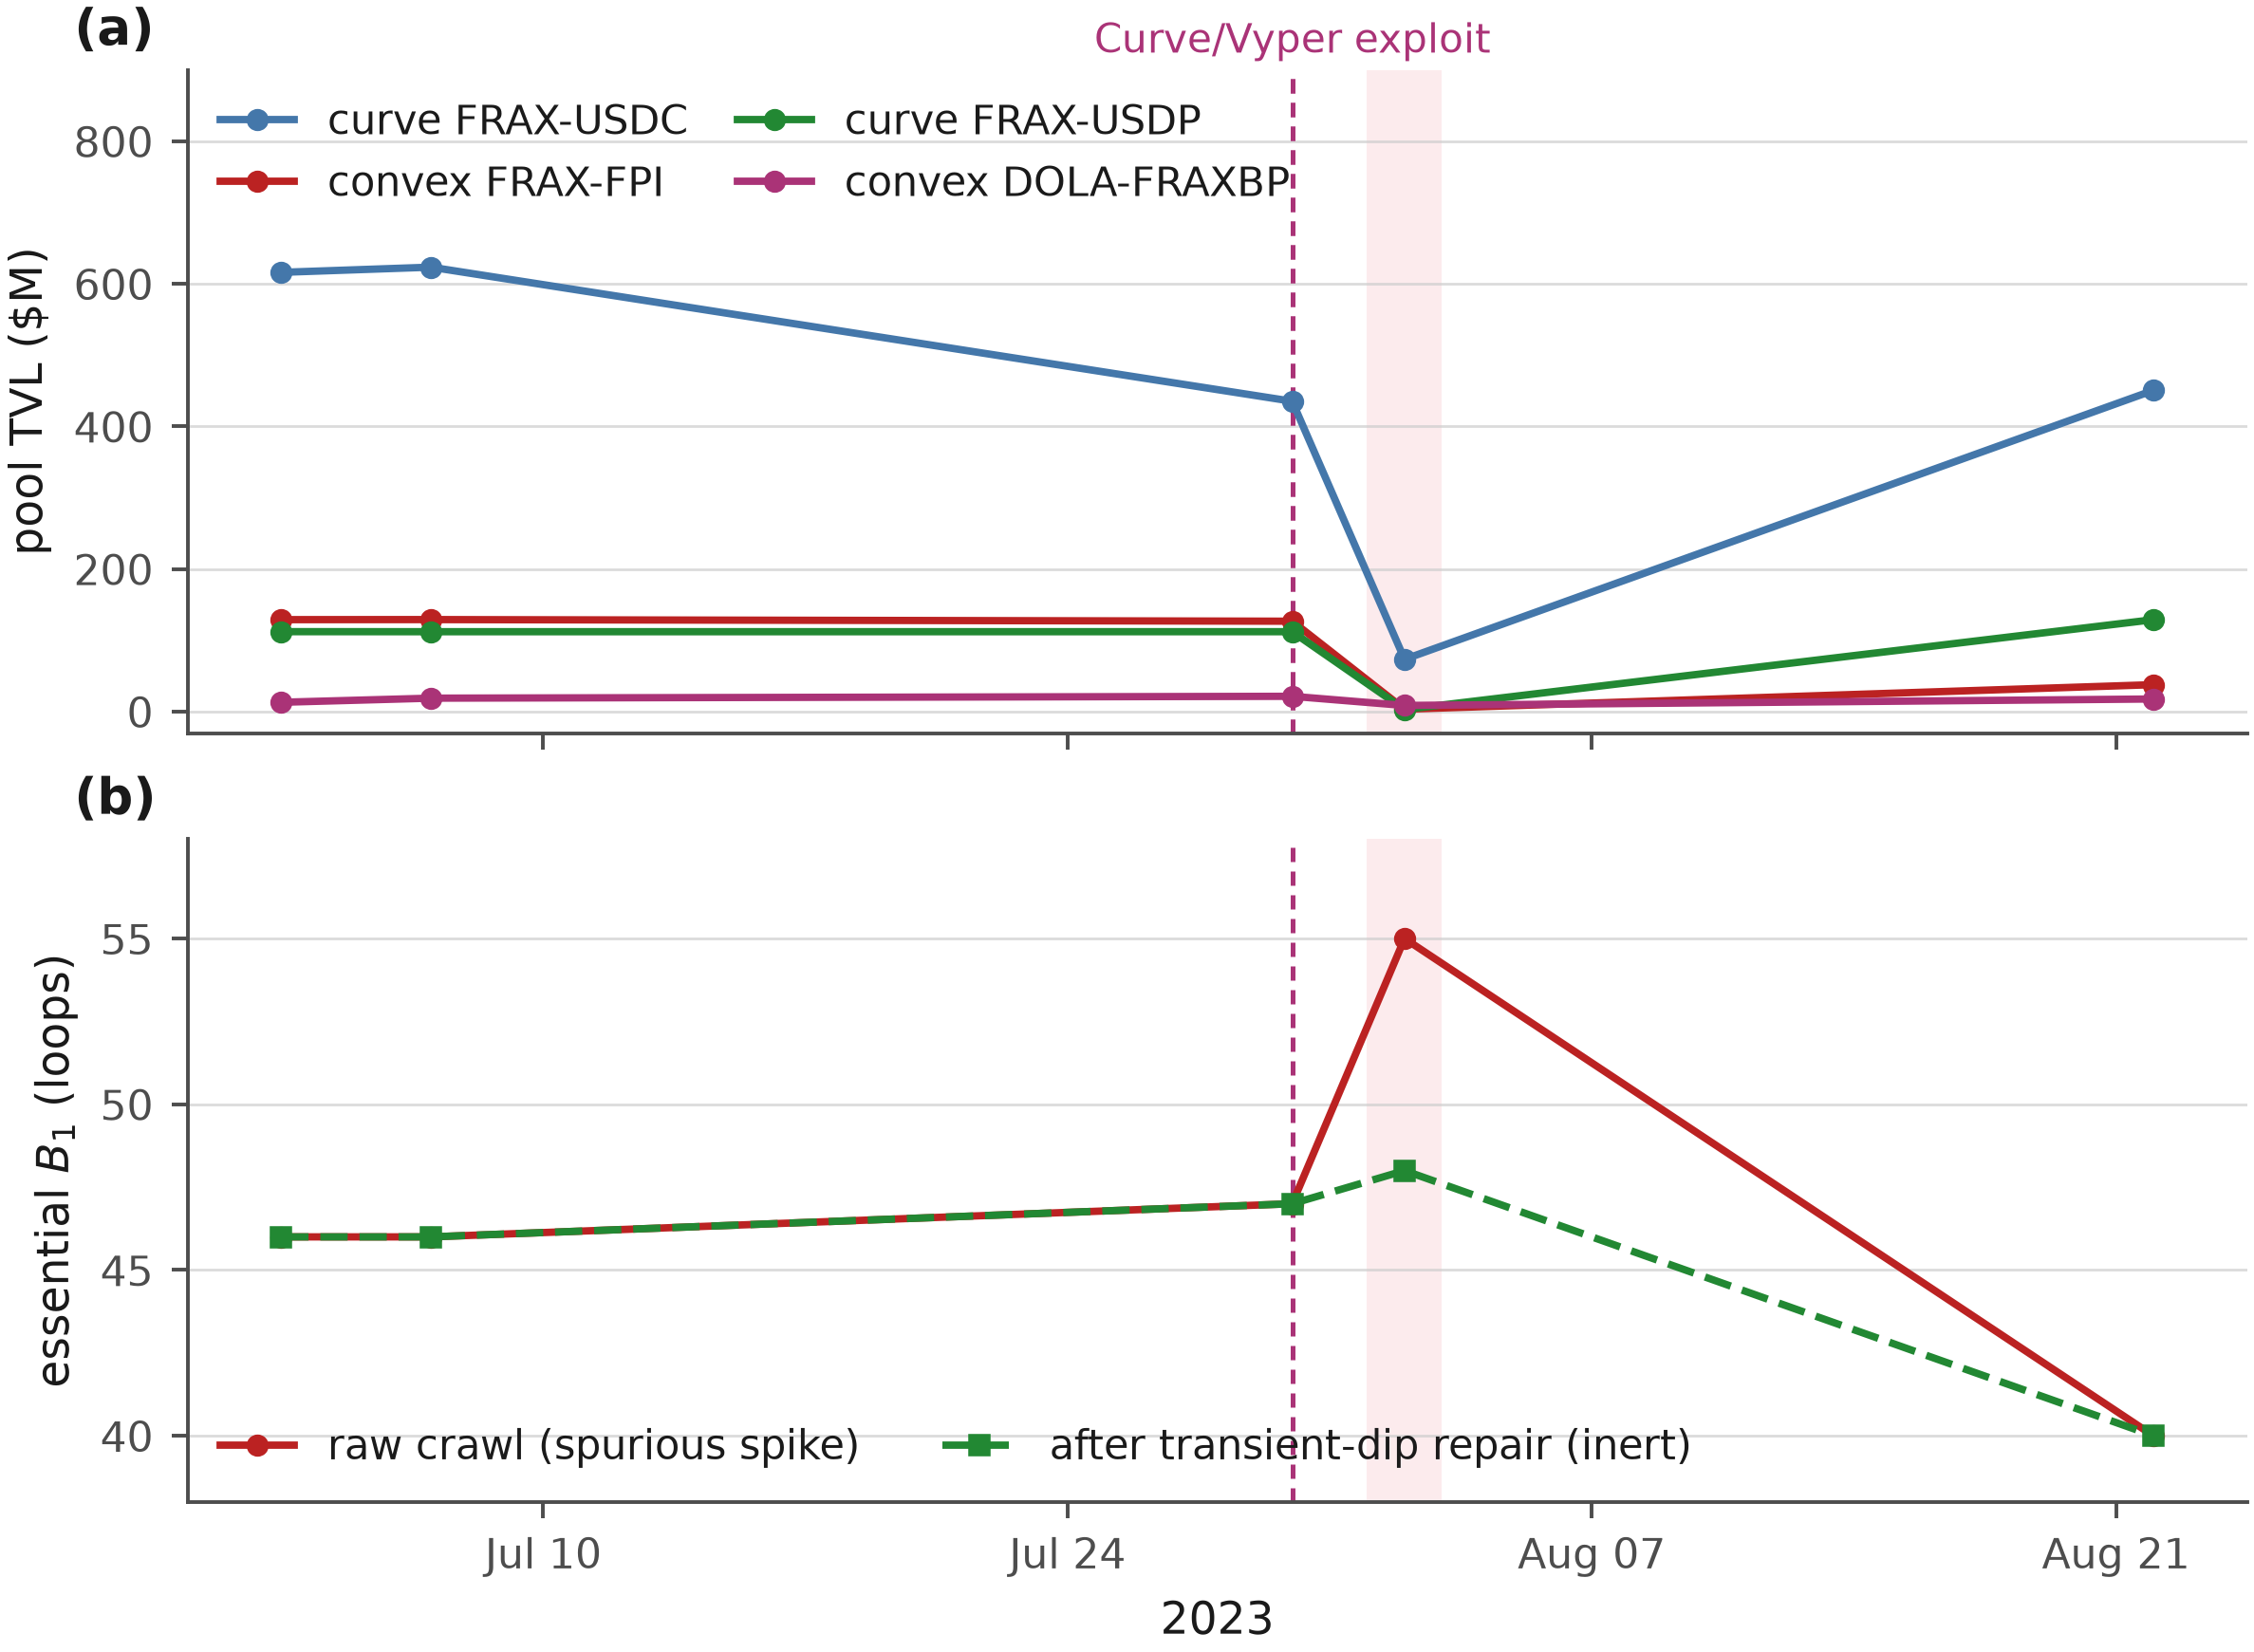
\includegraphics[width=\textwidth]{curve_artifact.png}
\caption{The Curve-exploit ``signal'' is a data glitch. \textbf{a} The pools driving the
apparent event crater to near-zero on the single 2023-08-02 crawl (shaded); three of the
four rebound to at or above their pre-event level within three weeks (FRAX-USDC
\$435M$\to$\$73M$\to$\$451M) and FRAX-FPI partially. A \$1.3B ``drawdown'' that reverses
on the next crawl is a reading error, not a liquidity event. \textbf{b} That corruption
injects a spurious essential-$B_1$ spike ($47\to55$, red) that transient-dip repair
removes ($\to48$, green), leaving the window stable. Dotted line: the exploit (2023-07-30);
the 10 dipped registry rows are 6 distinct pools, 8 rows of them FRAX.}
\label{fig:curve}
\end{figure*}

Unlike the descriptive fraction, the structural result holds under every choice we vary:
survivorship, LP representation, sampling cadence, and now two distinct stress events. It
directly refutes the natural objection that the survivor view looks rigid only through
omitting the pools that broke: restoring all 208 dead pools, the structure is still stable.

\subsection{How large a shock would have registered?}
\label{sec:inject}

\begin{figure*}[t]
\centering

\includegraphics[width=\textwidth]{injection.png}
\caption{What the event test could have seen. Starting from the depeg pre-event crawl
(274 pools, \$5.73B), pools are deleted synthetically and the change in essential $B_1$ is
recorded against the gap-matched detection threshold from Table~\ref{tab:null} (dashed).
Removing a random fifth of universe TVL, which costs about 60 pools, clears the threshold;
removing the same value concentrated in the largest pools does not, even at 70\percent.
The observable tracks how many pools are destroyed, not how much value. The star marks the
depeg as it actually occurred: 15 pools delisted, holding 0.8\percent\ of universe TVL,
roughly an order of magnitude below anything this test could resolve.}
\label{fig:inject}
\end{figure*}

A stability result on an integer-valued observable at weekly-to-monthly cadence invites an
obvious question: ``the structure did not move'' and ``this test cannot resolve a move this
small'' produce the same output. We separate them by damaging a real snapshot
synthetically and locating where essential $B_1$ leaves the band of routine drift.

From the 2023-03-07 crawl we delete pools three ways: the $N$ largest by TVL;
largest-first until $X$\percent\ of universe TVL is gone; and a random pool set totalling
the same $X$\percent, averaged over 12 seeds. Fig.~\ref{fig:inject} gives the
dose-response against the threshold of 5 loops.

The first result is that \textbf{the observable responds to pool count, not to value}.
Deleting the eight largest pools removes \SI{54}{\percent} of universe TVL and moves
essential $B_1$ by 3, under threshold; deleting a random fifth of TVL removes about 60
pools and moves it by 7. Targeted destruction stays under threshold to
\SI{70}{\percent} of TVL, while the diffuse threshold sits at \SI{20}{\percent} on all four
snapshots we repeated this on (2022-10, 2023-03, 2024-05, 2025-05). That is a property of
the nerve: a loop needs distinct pools weaving tokens together, and a large pool
contributes its own filled simplex as readily as its edges.

The second result \textbf{bounds the stability claim}. Across the depeg window 15 pools delisted,
holding \SI{0.8}{\percent} of universe TVL --- roughly an order of magnitude below
detectability in the dimension the observable actually responds to. Universe TVL did fall
\SI{24}{\percent} over the window, but almost all of that was repricing and outflow inside
pools that survived. So the reading in \S\ref{sec:disc}, that a depeg moves prices and
flows within a fixed scaffold rather than re-wiring it, is not only an interpretation
placed on the result: the injection test measures that mechanism directly, and the injection
also supplies the positive control the two observed events cannot provide. The bound is
specific to pool disappearance, which is the intervention a co-membership nerve is built to
see. A shock that re-wired membership without delisting anything is a different
intervention and falls outside the bound reported here.

\section{Discussion}
\label{sec:disc}

The representation sensitivity and the structural stability resolve under one economic
reading. Stablecoins are
near-perfect substitutes pegged to a common numéraire, so the liquidity network is a
hub-and-spoke around ``dollar-ness'' (mostly the 3pool and shallow wrappers) rather than
a rich web of distinct multi-way dependencies. Two consequences follow: (i) \emph{how much}
of that shallow scaffold counts as ``higher-order'' is set by the representation rather
than by the network: whether a metapool's dependence on the 3pool is one relationship (an
LP vertex) or three (resolved base assets) is a modeling stance, hence the 0.31--0.93
range; and
(ii) a depeg is prices and flows moving \emph{within} a fixed scaffold, not the scaffold
re-wiring, hence the stability.

The transferable lesson is methodological, and it is three traps deep. Registry-based
reconstruction is the default in empirical DeFi network research; it silently conditions on
survival (discarding $\sim$90\% of the loop structure), it hides an unremarked representation
choice (which, with survivorship, can flip a headline descriptive claim), and, as testing
the Curve exploit revealed, a crawl captured during an acute event can carry corrupted TVL
that \emph{manufactures} a topological signal. The last is the sharpest cautionary note: the
unguarded pipeline would have reported the FRAX-glitch spike as the sought-after ``topology
detects the exploit'' result. All three are cheap to address (de-censor via the Internet
Archive, report the representation sensitivity, and run an integrity scan with
transient-dip repair), but none is addressed by simply collecting more data. Where structural higher-order
TDA might still earn its keep is where these caveats bite less: non-substitute universes
(mixed collateral, cross-asset lending) with heterogeneous multi-way dependence, and slow
regime changes that actually re-wire membership.

\section{Limitations}
\begin{itemize}
\item \textbf{Two defensible conventions, no tie-breaker.} We report the range rather than
adjudicate; a reader with a specific economic question (exposure vs.\ composability) should
pick the matching convention and its number.
\item \textbf{Two de-censorable events, and no observed positive control.} The USDC depeg
and the Curve/Vyper exploit are both inside the archive window and both give the same
result, but
both are episodes where \S\ref{sec:disc} predicts membership should not re-wire, so on
their own they cannot show that the measure would respond to anything. Terra (May 2022)
predates the archive; the FTX collapse falls in a 31-day gap between crawls. The injection
test (\S\ref{sec:inject}) supplies a synthetic positive control in place of an observed
one: it establishes what \emph{pool deletion} of a given size does, rather than what a
re-wiring event would do. Spacing limits the test directly, leaving 15
gap-matched reference intervals. (A daily survivor-only placebo permutation reaches the
same result on the survivor sample; we report the de-censored version as primary evidence,
since \S\ref{sec:cnt} applies to the survivor view.)
\item \textbf{One data source, and it demonstrably fails.} Every quantity here is
DeFiLlama's, and \S\ref{sec:null} shows a single corrupted crawl nearly became the
headline finding. The integrity scan and transient-dip repair catch the failure mode we
found; they cannot certify the ones we did not. A registry error that is smooth across
neighbouring crawls, or a systematic mis-listing rather than a transient dip, would pass
both guards silently. Cross-checking TVL against an independent source (subgraph queries
or direct chain reads) is the obvious next hardening, and until it is done, single-source
risk is the largest uncosted exposure in the pipeline. A denser crawl cadence would also
tighten the event tests, which are currently spacing-limited (Table~\ref{tab:null}).
\item \textbf{Ethereum stablecoins only.} The economic reading (common-numéraire
substitutes) is exactly why the scaffold is shallow; other universes may differ, which is
the point.
\item \textbf{Cross-era representation.} The archive is natively lp\_vertex and today's API
resolved; we run both explicitly rather than mixing them.
\end{itemize}

\section{Conclusion}

Measured rather than asserted, the higher-order structure of Ethereum stablecoin liquidity
has no representation-invariant size: the higher-order fraction ranges 0.31--0.93 across two
modeling choices, LP-token representation (the larger) and survivorship, that
registry-based DeFi network studies routinely leave unexamined, and even its time-trend flips sign
between conventions. Survivor-only reconstruction, the field default, sees roughly a tenth
of the loop structure; Internet-Archive de-censoring recovers the rest and revives an
otherwise-untestable representation fork. The one representation-independent structural
result is stability, and it is bounded: through both the largest stablecoin depeg on record
and the Curve/Vyper exploit an event window looks like any other window of its length, and
synthetic damage puts the detection floor near a fifth of the universe against a depeg
that delisted \SI{0.8}{\percent} of it. Reaching that conclusion required catching a third
trap, a corrupted event-window crawl that would
otherwise have read as a spurious detection. Report higher-order DeFi structure as a
sensitivity range, de-censor the registry, scan for event-window data corruption, and read
the structural result off the dynamics, which are stable, with the levels reported as the
range they are.

\section*{Reproducibility}
All code, the computed observable series, and figures are at
\url{https://github.com/adamLEVi16/topology-engine} (\texttt{defi\_topology/}). The pipeline
runs from the free DeFiLlama API and the Internet Archive with no authentication; the raw
registry snapshots ($\sim$390\,MB) are re-fetched rather than committed. Since the
Wayback Machine is append-only, resolving a target date to its ``closest crawl'' can drift
over time, so the exact snapshot timestamps used are recorded in the series JSON and the
series is rebuilt byte-for-byte with \texttt{decensor.py --pinned} (each timestamp maps to a
fixed, permanent crawl). Toy-complex tests pin the topology, and every number is regenerated
by a single script per result (\texttt{decensor.py} for the de-censored series, the
2$\times$2, the event tests,
and the integrity scan / \texttt{repair\_transient\_dips} data-quality guard).

\begin{thebibliography}{9}
\small
% External identifiers are hyperlinked via \doi / \arxiv (defined in the preamble). Every
% DOI below was checked against Crossref and every arXiv id against the arXiv API; nothing
% here is a guessed identifier.
\bibitem[Aufiero et al.(2025)]{tradefidefi2025} Aufiero, S., Bartolucci, S.,
Caccioli, F., Vivo, P. (2025). Mapping microscopic and systemic risks in TradFi and
DeFi: a literature review. \arxiv{2508.12007}.
\bibitem[Bick et al.(2023)]{bick2023} Bick, C., Gross, E., Harrington, H.~A., Schaub,
M.~T. (2023). What are higher-order networks? \emph{SIAM Review} 65(3), 686--731.
\doi{10.1137/21M1414024}.
\bibitem[de Favereau de Jeneret \& Diamantis(2025)]{fx2025} de Favereau de Jeneret,
P., Diamantis, I. (2025). Topology of currencies: persistent homology for FX
co-movements: a comparative clustering study. \arxiv{2510.19306}.
\bibitem[Eisenberg \& Noe(2001)]{eisenberg2001} Eisenberg, L., Noe, T.~H. (2001).
Systemic risk in financial systems. \emph{Management Science} 47(2), 236--249.
\doi{10.1287/mnsc.47.2.236.9835}.
\bibitem[Forte(2026)]{forte2026} Forte, F.~D. (2026). It takes two to tango, but more
to assess systemic risk: credit networks through the lens of hypergraphs.
\arxiv{2607.10943}.
\bibitem[Gidea \& Katz(2018)]{gidea2018} Gidea, M., Katz, Y. (2018). Topological data
analysis of financial time series: landscapes of crashes. \emph{Physica A} 491,
820--834. \doi{10.1016/j.physa.2017.09.028}.
\bibitem[Yan \& Tessone(2025)]{uniswap2025} Yan, T., Tessone, C.~J. (2025). Network
analysis of Uniswap: centralization and fragility in the decentralized exchange
market. \arxiv{2503.07834}.
\end{thebibliography}

\end{document}
